
%(BEGIN_QUESTION)
% Copyright 2010, Tony R. Kuphaldt, released under the Creative Commons Attribution License (v 1.0)
% This means you may do almost anything with this work of mine, so long as you give me proper credit

PT-58, PRC-58, and PV-58 comprise a gas pressure control system to monitor and regulate gas pressure in this oil/natural-gas separator vessel by venting excess natural gas to the flare.  During normal operation, there is just a little bit of gas flow vented to the flare.  Most of the gas exits the separator vessel through control valve FV-66:

$$\includegraphics[width=15.5cm]{i03708x01.eps}$$

Suppose one day an instrument technician shuts the high-side block valve and opens the equalizing valve on the three-valve manifold attached to PT-58, while the system is operating under normal conditions as described above.  Determine the effect of this valve manifold change on the actual gas pressure and actual liquid level inside the separator vessel, explaining your reasoning for both.

\underbar{file i03708}
%(END_QUESTION)





%(BEGIN_ANSWER)

\noindent
5 points for each correctly-reasoned answer:

\vskip 10pt

Gas pressure will {\bf rise} inside the separator vessel because the PRC-58 will see 0 pressure inside the vessel with PT-58 blocked and equalized.  

\vskip 10pt

Liquid level will {\bf remain unchanged}, as LT-83 and LC-83 will continue to operate normally.

%(END_ANSWER)





%(BEGIN_NOTES)

{\bf This question is intended for exams only and not worksheets!}.

%(END_NOTES)


